\documentclass[fleqn,oneside,a4]{article}
\newcommand{\level}{\section}
\newcommand{\sublevel}{\subsection}
\newcommand{\subsublevel}{\subsubsection}

% \documentclass[fleqn,oneside,a4]{book}
% \newcommand{\level}{\chapter}
% \newcommand{\sublevel}{\section}
% \newcommand{\subsublevel}{\subsection}

\usepackage{algorithm2e}
\usepackage{amsmath}
\usepackage{amsthm}
\usepackage{amssymb}
\usepackage{color}
\usepackage{dsfont}
\usepackage{enumitem}
\usepackage{graphicx}
\usepackage{listings}
\usepackage{mathtools}
\usepackage{makeidx}
\usepackage{multicol}
\usepackage{tikz-cd}

\hoffset = 0pt
\voffset = 0pt
\oddsidemargin = 0pt
\evensidemargin = 0pt
\topmargin = 0pt
\headsep = 0pt
\textheight = 650pt
\textwidth = 450pt

% Soft colors.

% \definecolor{red}{rgb}{0.8,0.1,0.1}
% \definecolor{blue}{rgb}{0.1,0.2,0.8}

% Some useful definitions.

\newcommand{\comment}[1]{\textcolor{blue}{#1}}  % red
\newcommand{\Lra}{\Leftrightarrow}
\newcommand{\nat}{\mathds{N}}
\newcommand{\new}[1]{\textcolor{black}{#1}}  % blue
% \newcommand{\new}[1]{\fcolorbox{black}{white}{#1}}
\newcommand{\ol}{\overline}
\newcommand{\pcunchanged}{c_{t + 1} = c_t}
\newcommand{\Ra}{\Rightarrow}
\newcommand{\ra}{\rightarrow}
\newcommand{\term}[1]{\textit{#1}\index{#1}}
% \newcommand{\term}[1]{\textcolor{magenta}{#1}}
\newcommand{\true}{\textbf{true}}
\newcommand{\false}{\textbf{false}}

% Execution marks

\newcommand{\te}[1]{#1^T}      % Taint execution
\newcommand{\se}{\overline}    % Symbolic execution
\newcommand{\dse}{\widetilde}  % Dynamic symbolic execution

% Assert, declare and update as commands.

\newcommand{\assert}{\textbf{assert}\,}
\newcommand{\declare}{\textbf{declare}\,\,}
\newcommand{\update}{\textbf{update}\,\,}

% Assert, declare and update as statements.

% \newcommand{\assert}{c_{t + 1} = c_t \cup}
% \newcommand{\declare}{}
% \newcommand{\update}{}

\newcommand{\lblock}{ \left \{ \begin{array}{l} }
\newcommand{\rblock}{ \end{array} \right. }

\renewcommand{\arraystretch}{1.5}
\renewcommand\qedsymbol{$\blacksquare$}

\newtheorem{theorem}{Theorem}
\newtheorem{lemma}[theorem]{Lemma}
\newtheorem{claim}{Claim}

\lstset{
    basicstyle=\linespread{0.9}\small\ttfamily,
    keywordstyle=\bfseries\color{black},
    stringstyle=\color{black},
    identifierstyle=\color{black}
}

\setlength{\parindent}{0em}

\title{Formal model of concrete, symbolic,
    dynamic symbolic execution (concolic execution),
    and taint tracking}
\author{Sergey Vartanov}
\makeindex

\begin{document}

\maketitle

% \setlength{\parskip}{0em}
%
% \tableofcontents
%
% \pagebreak

\setlength{\parskip}{0.5em}

The main goal of this document is to propose a formal definition of
some program analysis terms, such as execution (concrete execution),
(pure) symbolic execution,
dynamic symbolic execution (concolic execution),
feasibility, and taint analysis.

\level{Concrete program execution}

\sublevel{Program definition}

\term{Program} is defined by functional elements and data:
    $\mathcal{P} = \langle F, F_I, F_T, D \rangle$.
Where function elements and data defined as followed:
\begin{itemize}
    \item $F = \{f_j\} = \{(f^F_j, f^D_j)\}$~is \term{function element} set.
        $f_j: D \ra F \times D$~is \term{function element}.
        $f_j = (f^F_j, f^D_j)$:
        \begin{itemize}
            \item $f^F_j: D \ra F$~is
                \term{control flow function element}.
            \item $f^D_j: D \ra D$~is \term{data flow function element}.
        \end{itemize}
        Function element could be considered as program instruction, that
        computes next program instruction \{$f^F_j$\}
        and modifies data \{$f^D_j$\}.
    \item $F_I$ is a set of \term{initial function elements}.
    \item $F_T$ is a set of \term{terminal function elements}.
    \item $D = \{d_j\}$ is \term{data}, $d_j \in \mathcal{B}$, which is
        \term{data set}.
\end{itemize}

Additionally, we will assume the following.
\begin{itemize}
    \item Program is not empty: $F \neq \varnothing$.
    \item $\forall j \,\, f^F_j$ is a total function.
    \begin{itemize}
        \item If $f_j \notin F_T$,
            $\forall d \in D \,\, f^F_j(d) = f_k, f_k \in F$.
        \item If $f_j \in F_T$,
            $\forall d \in D \,\, f^F_j(d) = f_j$.
    \end{itemize}
    \item To simplify considering, we will assume that unless otherwise stated
        there is one and only one initial function element $f_0$:
        $F_I = \{f_0\}$.
    \item Program has at least one terminal function elements:
        $F_T \neq \varnothing$.
\end{itemize}

\subsublevel{Limitations}

We assume \textbf{deterministic} program execution
using \textbf{limited} binary data without \textbf{self-modification}.
Concrete program execution means normal program execution on given binary data.

\begin{itemize}
    \item Firstly, we should emphasize that we distinguish data ($D$)
        from function elements ($F$).
        It implies that self-modification is not possible.
        To allow self-modification, we should merge $F$ and $D$ into one set.
    \item Program is deterministic: $f^F_j: D \ra F$.
        For nondeterministic program it should be: $f^F_j: D \ra F*$.
    \item Data is limited and predefined: $|D| < \infty$.
\end{itemize}

\subsublevel{Possible data model definition}

Data ($D$) and data set ($\mathcal{B}$) are abstract sets.
But for further consideration we will use a number of
possible data and data set definitions.

Binary data:
\begin{itemize}
    \item $B = \{0, 1\}, \mathcal{B}_2 = B^8$.
\end{itemize}

Data model definition with registers and memory:
\begin{itemize}
    \item $D_1 = \{d_j\} = R \cup M$.
    \begin{itemize}
        \item $R = \{r_j\}$~--- \term{concrete registers}.
            $r_j \in \mathcal{B}_2$.
        \item $M = \{m_j\}$~--- \term{concrete memory}. $m_j \in \mathcal{B}_2$.
    \end{itemize}
\end{itemize}

For the next data model definition we will
\textbf{avoid limited data condition}.
Here $Y$ is a set of sets $Y_i$.
Each set $Y_i$ may contain an arbitrary number of elements.
Data model definition with set of inputs, registers, memory,
and external knowledge about array allocation:
\begin{itemize}
    \item $D_2 = \{d_j\} = Y \cup R \cup M \cup L$. $|L| \le |M|$.
    \begin{itemize}
        \item $Y = \{Y_i\}$~--- \term{concrete inputs},
            $Y_i = \{y_{i, j}\}$~--- \term{concrete input}.
            $y_{i, j} \in \mathcal{B}_2$.
        % \item $Y = \{ Y_i \}$~--- \term{inputs},
        %     $Y_i = \langle \{y_{i, j}\}, y_{i, l} \rangle$~--- \term{input}.
        %     $y_{i, j} \in \mathcal{B}_2, y_{i, l} \in \mathcal{B}_2$.
        \item $R = \{r_j\}$~---
            \term{concrete registers}. $r_j \in \mathcal{B}_2$.
        \item $M = \{m_j\}$~---
            \term{concrete memory}. $m_j \in \mathcal{B}_2$.
        \item $L = \{l_j\}$~---
            \term{concrete array lengths}. $l_j \in \mathcal{B}_2$.
    \end{itemize}
\end{itemize}

\subsublevel{Control flow graph}

Set of next possible function elements for function element $f$ is
$f[D] = \{f_j \in F | f_j = f^D(d), d \in D\}$.
\term{Control flow graph} is a directed graph where vertices
are function elements and there is an edge from
vertex $f_i$ to vertex $f_j$ iff $f_j \in f_i[D]$.
Function element $f_j = (f_j^F, f_j^D)$ is \term{branch} iff $|f_j[D]| > 1$.
Otherwise (if range of the control flow function
element has exactly one element),
function element is \term{operation},
i.e. iff $\exists f_k: f_j^D(d) = f_k, \forall d \in D$.

The set of all branches is $F_B: \{f_j \in F: |f_j[D]| > 1\}$.
The set of all operations is $F_O: \{f_j \in F: |f_j[D]| = 1\}$.
Since $|f_j[D]|$ by definition is either equals to 1, or greater than 1,
$F = F_B \cup F_O$ and $F_B \cap F_O = \varnothing$.

We will use graphical representation of control flow graph using circles
for vertices with function element captions and arrows for edges.
Vertices that correspond to terminal function elements will be represented
by circles with double stroke.
Vertices that correspond to initial function elements will be represented
as usual.
We assume that either there is a single initial element $f_0$,
or initial elements are represented by vertices that has no incoming edges.

\sublevel{Execution}

We consider that program execution is an iterative process with steps.
For further considerations we will use variable $t \in \nat$ as
\term{execution step}.
At every step program execution has its \term{program state} $s = (f, d)$:
next function element (next instruction) and current \term{data state}.
$f \in F, d \in D$.
Set of all possible execution states is $S$.
Program state at the iteration $t$ is
$s_t = (f_t, d_t) = \big((f_t^F, f_t^D), d_t\big)$.
$(f_0, d_0), f_0 \in F_I$ is \term{initial state}.
Any state $(f_t, d_t)$ such as $f_t \in F_T$ is \term{terminal state}.

We consider that there is \term{execution function} $\mathcal{F}: S \ra S$
that manages the execution process:
$$\mathcal{F}(s_t) = \mathcal{F}\big((f_t, d_t)\big) =
    f_t(d_t) =
    \big(f_t^F(d_t), f_t^D(d_t)\big) =
    (f_{t + 1}, d_{t + 1}) = s_{t + 1}.$$

Execution function $\mathcal{F}$ defines an \term{execution rule}:
\begin{itemize}
    \item $f_{t + 1} = f_t^F(d_t)$,
    \item $d_{t + 1} = f_t^D(d_t)$.
\end{itemize}

\term{Execution of a program} $\mathcal{P} = \langle F, F_I, F_T, D \rangle$
on \term{input data} $d_0$, where $F_I = \{f_0\}$,
is a chain of program states,
starting with initial state $s_0 = (f_0, d_0)$,
where next state is a function $\mathcal{F}$ of previous state:
$$s_{t + 1} = (f_{t + 1}, d_{t + 1}) = \big(f_t^F(d_t), f_t^D(d_t)\big) =
    \mathcal{F}(s_t), s_t \in S$$
and either none of function elements.

We consider that if program execution approaches state $s_t = (f_t, d_t)$,
where $f_t \in F_T$, program execution is terminated.
Hence, execution is either infinite chain
$$E(d_0) = s_0 \ra s_1 \ra \cdots \ra s_t \ra \cdots =
        (f_0, d_0) \ra (f_1, d_1) \ra \cdots \ra (f_t, d_t) \ra \cdots,$$
where $\forall j \,\, f_j \notin F_T$ (in this case $d_t$ is an
\term{output data} of program execution $E(d_0)$),
or finite chain
$$E(d_0) = s_0 \ra s_1 \ra \cdots \ra s_t =
        (f_0, d_0) \ra (f_1, d_1) \ra \cdots \ra (f_t, d_t),$$
where $f_t \in F_T \land \forall j < t \,\, f_j \notin F_T$
(in this case execution has no output data).
For the first case we will use notation $E(d_0) \ra d_t$,
for the second: $E(d_0) \ra \infty$.

\begin{lemma}
    \label{exists_one_execution}
    $\forall \mathcal{P} = \langle F, F_I, F_T, D \rangle \,\,
    \forall d \in D \,\, \exists! E(d)$.
\end{lemma}

\begin{proof}
    Let's prove it by constructing the execution chain.
    By the program definition, there is a initial function element $f_0$.
    Hence, $\forall d \in D$
    there is a initial program state $s_0 = (f_0, d)$.
    For every program state $s_t = (f_t, d_t)$,
    either $f_t \notin F_T \Ra f_t(d_t) = (f_{t + 1}, d_{t + 1})$
        and we have next step of the execution,
    or $f_t \in F_T \Ra$ execution is terminated.
    All steps of this process are deterministic,
    hence we will have execution $E(d)$ determined by initial input data $d$.
\end{proof}

To visualize the process of the program execution we will use circles
for program states connected by arrows which depicts function $\mathcal{F}$.
If program execution is finite, the last state will be depicted by
a circle with double stroke.

\begin{figure}[h!]
    \begin{center}
        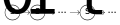
\includegraphics[scale=1.25]{image/concrete_execution.pdf}
    \end{center}
    \caption{Infinite and finite concrete program execution}
\end{figure}

We will also define \term{execution path} as either any finite sequence
$P = \{f_0, f_1, \dots, f_t\}$, where
$\forall j \,\, f_j \in F \land f_{j + 1} \in f_j[D]$
and $f_t \in F_T \land \forall j < t \,\, f_j \notin F_T$
or infinite sequence $P = \{f_0, f_1, \dots, f_t, \dots\}$, where
$\forall j \,\, f_j \in F \land f_{j + 1} \in f_j[D] \land f_j \notin F_T$.

\begin{lemma}
    There is one and only one execution path $P$ for the execution $E(d_0)$.
    \[ \begin{array}{c}
    \forall E(d_0) = s_0 \ra s_1 \ra \cdots \ra s_t \ra \cdots =
        (f_0, d_0) \ra (f_1, d_1) \ra \cdots \ra (f_t, d_t) \ra \cdots \\
    \exists! P = \{f'_0, f'_1, \dots, f'_t, \dots\}:
        f'_0 = f_0, f'_1 = f_1, \dots, f'_t = f_t, \dots
    \end{array} \]
\end{lemma}

\begin{proof}
    Let's create an array $P = \{f_0, f_1, \dots, f_t, \dots\}$ from
    execution states.
    Now we have to proof that $P$ is execution path.
    Choose arbitrary $f_j = (f_j^F, f_j^D)$ and $f_{j + 1}$.
    By execution definition,
    $f_{j + 1} = f_j^F(d_j) \Ra f_{j + 1} \in f_j[D]$.
    Hence, $P$ is an execution path.
\end{proof}

We will denote this fact as $E(d_0) \Ra P$.

Let's also define a \term{branch chain} $P_B$ of a execution path $P$
as a subsequence of $P$, which contains only $f_j \in F_B$.
We can denote this fact as $P \Ra P_B$

% $P_B = \{f_{j_0}, f_{j_1}, \dots, f_{j_k}, \dots\}$, where
% $\forall k \,\, f_{j_k} \in F_B$

\begin{lemma}
    $\forall P_B \,\, \exists! P: P \Ra P_B$.
\end{lemma}

\begin{proof}
    \comment{Add proof.}
\end{proof}

Therefore, we can write $P \Lra P_B$.

Note, that we define execution path just as a path in control flow graph.
It could be infeasible if there is no such input data that implies that path.
Execution path $P$ is \term{feasible in concrete model} iff
$\exists d_0 \in D: (f_1, d_1) = f_0(d_0) \land
    \forall j > 0 ~ (f_j, d_j) = f_{j - 1}(d_{j - 1})$.

Some sets of program executions:
\begin{itemize}
    \item $\mathds{E}_\mathcal{P}$~--- set of all possible program executions.
    \item $\mathds{P}_\mathcal{P}$~--- set of all possible execution paths.
        $\mathds{P}'_\mathcal{P}$~---
        set of all possible feasible execution paths.
\end{itemize}

\subsublevel{Number of paths}

\begin{lemma}
    $|\mathds{E}_\mathcal{P}| = |D| |\mathcal{B}|$.
\end{lemma}

\begin{proof}
    $|D| |\mathcal{B}|$~--- number of all possible data states.
    From lemma \ref{exists_one_execution},
        $\forall d \in D \,\, \exists! E(d)$.
    $\forall d', d'' \in D : d' \neq d'' \,\, E(d') = (f_0, d') \ra \cdots
        E(d'') = (f_0, d'') \ra \cdots.
        (f_0, d') \neq (f_0, d'') \Ra E(d') \neq E(d'').$
    Therefore, number of possible executions is equal to number of
    possible initial input data.
\end{proof}

\begin{lemma}
    $|\mathds{P}_\mathcal{P}| = \infty$.
    $|\mathds{P}''_\mathcal{P}| \le |D| |\mathcal{B}|$.
\end{lemma}

\level{Symbolic execution model}

Symbolic execution of the program is
an execution of a symbolic model of that program.
Symbolic model includes a set of symbolic function element
(symbolic models of function elements) and
symbolic data model.
Execution is performed using symbolic variables instead of concrete data.

\sublevel{Model}

$\se{\mathcal{P}} = \langle \se{F}, \se{F}_I, \se{F}_T, \se{D} \rangle$~---
\term{symbolic model} of program
$\mathcal{P} = \langle F, F_I, F_T, D \rangle$.
There are a lot of ways to create a symbolic model from the program,
therefore we will use some particular set of rules $R_\text{SE}$.
We can write it as
$\mathcal{P} \xrightarrow[]{R_\text{SE}} \se{\mathcal{P}}$.
It denotes that for all $\mathcal{P}$ exists only one symbolic model
$\se{\mathcal{P}}$ constructed using the set of rules $R_\text{SE}$.

From definition:
\begin{itemize}
    \item $\se{F} = \{\se{f}_j\} =
        \{(\se{f}_j^F, \se{f}_j^D, \se{f}_j^C)\}$~---
        \term{symbolic function element models}
        that correspond to function elements of the program $\mathcal{P}$.
    \item $\se{F}_I$ is a set of
        \term{initial symbolic function element models},
        that correspond to initial function elements
        of the program $\mathcal{P}$.
    \item $\se{F}_T$ is a set of
        \term{terminal symbolic function element models},
        that correspond to terminal function elements
        of the program $\mathcal{P}$.
    \item $\se{f}_j: \se{D} \times C \ra
        (\se{F} \times \se{D} \times C)*$~---
        \term{symbolic function element model}:
    % %%% Not sure we have to divide function $\se{f}_j$.
    % \begin{itemize}
    %     \item $\se{f}_j^F: \varnothing \ra \se{F}*$~---
    %         \term{control flow symbolic function element model},
    %     \item $\se{f}_j^D: \se{D} \ra \se{D}*$~---
    %         \term{data symbolic function element model}.
    %     \item $\se{f}_j^C: \se{D} \times C \ra C*$~---
    %         \term{data symbolic function element model}.
    % \end{itemize}
    % \end{itemize}
\end{itemize}

\subsublevel{Data model}

Data model with memory, registers, and array lengths.

\begin{itemize}
    \item $\se{D} = \{\se{d}_j\} = \se{R} \cup \new{\se{M}} \cup \se{L}$~---
        \term{symbolic data model}.
    \begin{itemize}
        \item $\se{R} = \{\se{r}_j\}, \se{r}_j = x_r, x_r \in X_R$~---
            \term{symbolic registers model}.
        \item $\se{M} = \{\se{m}_j\}, \se{m}_j = x_m, x_m \in X_M$~---
            \term{symbolic memory model}.
        \item $\se{L} = \{\se{l}_j\}, \se{l}_j = x_l, x_l \in X_L$~---
            \term{symbolic length model}.
    \end{itemize}
    \item $X = X_M \cup \new{X_L} \cup X_R$.
    \begin{itemize}
        \item $X_M = \{x_m\}$~---
            \term{memory symbolic variables}. $x_m \in \mathcal{B}$.
        \item \new{$X_L = \{x_l\}$~--- \term{length symbolic variables}.
            $x_l \in \mathcal{B}$.}
        \item $X_R = \{x_r\}$~---
            \term{register symbolic variables}. $x_r \in \mathcal{B}$.
    \end{itemize}
\end{itemize}

\sublevel{Execution}

Symbolic execution unlike concrete execution is not an iterative process.
However, it has execution states
$\se{s} = (\se{f}, \se{d}, c)$~--- \term{symbolic state},
$\se{f} \in \se{F}, \se{d} \in \se{D}, c \in C$.
Set of all possible symbolic states is $\se{S}$.
$(\se{f}_0, \se{d}_0, \varnothing)$ is an \term{initial symbolic state}.
Any state $(\se{f}_t, \se{d}_t, c_t)$, such as $\se{f}_t \in \se{F}_T$
is a \term{symbolic terminal state}.
Note, that $t$ is not an execution step here, but a state identifier.

We consider that there is a \term{symbolic execution function}
$\se{\mathcal{F}}: \se{S} \ra \se{S}$
that manages the symbolic execution process:

\begin{align*}
\se{\mathcal{F}}(s_{k, \dots, l})
&= \se{\mathcal{F}}
    \big((f_{k, \dots, l}, d_{k, \dots, l}, c_{k, \dots, l})\big) = \\
&= \{(f_{k, \dots, l, m}, d_{k, \dots, l, m}, c_{k, \dots, l, m}), \dots, 
       (f_{k, \dots, l, n}, d_{k, \dots, l, n}, c_{k, \dots, l, n})\} = \\
&= \{s_{k, \dots, l, m}, \dots, s_{k, \dots, l, n}\}
\end{align*}

Definitions:
\begin{itemize}
    \item $C = \{e_i\}$~--- \term{path condition} or \term{path constraint}.
    \item $X = \{x_k\}, x_k \in \mathcal{B}$~--- \term{symbolic variables}.
\end{itemize}

\begin{itemize}
    \item $\se{E} = \se{s}_0 \ra \cdots$ \comment{add picture}~--- pure
        symbolic execution.
\end{itemize}

\begin{tikzcd}
    && \se{s}_{0,0,0} \arrow{r} & \cdots \\
    & \se{s}_{0,0} \arrow{ru} \arrow{r} \arrow{rd} & \cdots \\
    \se{s}_0 \arrow{r} \arrow{ru} \arrow{rd} & \cdots & \se{s}_{0,0,n_{0,0}}
        \arrow{r} & \cdots \\
    & \se{s}_{0,n_0} \arrow{r} & \cdots
\end{tikzcd}

Execution rule:
\begin{itemize}
    \item $\{\se{f}_{0, t_1, \dots, t_n, 0}, \dots,
            \se{f}_{0, t_1, \dots, t_n, m}\} =
        \se{f}_{0, t_1, \dots, t_n}^F(\se{d}_{0, t_1, \dots, t_n})$,
    \item $\{\se{d}_{0, t_1, \dots, t_n, 0}, \dots,
            \se{d}_{0, t_1, \dots, t_n, m}\} =
        \se{f}_{0, t_1, \dots, t_n}^D(\se{d}_{0, t_1, \dots, t_n})$.
\end{itemize}

Execution path $P = \{\se{f}_0, \se{f}_1, \dots, \se{f}_t\}$ is
\term{feasible in symbolic model} iff $c_{0, 1, \dots, t}$ is true.

\sublevel{Symbolic execution and concrete execution}

\comment{Feasibility in concrete model vs feasibility in symbolic model.}

\level{Taint tracking}

\sublevel{Model}

Binary taint tracking:

\begin{itemize}
    \item $\mathcal{T}$ is a set of possible taint marks.
        E.g. $\{\textbf{false}, \textbf{true}\}, \nat$, etc.
    \item $T = \{\tau_j\}$~--- taint set.
    \item $\te{D}$~--- taint data model.
    \begin{itemize}
        \item $\te{M} = \{\te{m}_j\}, \te{m}_j \in \mathcal{T}$~---
            \term{taint memory model},
        \item $\te{R} = \{\te{r}_j\}, \te{r}_j \in \mathcal{T}$~---
            \term{taint registers model}.
    \end{itemize}
\end{itemize}

\level{Dynamic symbolic (concolic) execution model}

\sublevel{Model}

Definitions:
\begin{itemize}
    \item $\dse{\mathcal{P}} = \langle F, F_I, F_T, D,
        \se{F}, \se{F}_I, \se{F}_T, \se{D} \rangle$~---
        concolic model of program
        $\mathcal{P} = \langle F, F_I, F_T, D \rangle$
        and its symbolic model
        $\se{\mathcal{P}} =
            \langle \se{F}, \se{F}_I, \se{F}_T, \se{D} \rangle$.
        \item $Y = \{Y_i\}$~--- \term{taint sources}.
              $Y_i = (\{y_{i_j}\}, \new{y_{i_L}})$,
              $y_{i_j} \in \mathcal{B}$~--- \term{taint source elements},
              \new{$y_{i_L} \in \mathcal{B}$~--- \term{taint source size}}.
\end{itemize}

\sublevel{Execution}

Dynamic symbolic execution or, in other words, concolic execution,
is an execution of a program along with execution of its symbolic model
(that means construction of a path condition) but for the particular
execution path that is defined by initial input data $d_0$.

As a concrete execution, it is iterative process with steps.
We will also use variable $t \in \nat$ as execution step.
At every step, there are program execution state $s_t = (f_t, d_t)$
and symbolic execution state $\se{s}_t = (\se{f}_t, \se{d}_t, c_t)$,
which we combine into \term{concolic state}
$\dse{s}_t = (f_t, d_t, \se{f}_t, \se{d}_t, c_t)$.

We consider that there is Dynamic symbolic execution function
$\dse{\mathcal{F}}: \dse{S} \ra \dse{S}$
that manages the execution process:
\begin{align*}
\dse{\mathcal{F}}(\dse{s}_t) &=
    \dse{\mathcal{F}}\big((f_t, d_t, \se{f}_t, \se{d}_t, c_t)\big) = \\
    &= (f_t^F(d_t), f_t^D(d_t),
        \se{f}_t^F(\se{d_t}), \se{f}_t^D(\se{d_t}), c_{t + 1}) = \\
    &= (f_{t + 1}, d_{t + 1}, \se{f}_{t + 1}, \se{d}_{t + 1}, c_{t + 1}) = \\
    &= \dse{s}_{t + 1}.
\end{align*}

\comment{Add function to produce $c_{t + 1}$ from $c_t$.}

Execution function $\mathcal{F}$ defines an \term{execution rule}:
\begin{itemize}
    \item $f_{t + 1} = f_t^F(d_t)$,
    \item $d_{t + 1} = f_t^D(d_t)$.
\end{itemize}

\term{Dynamic symbolic execution} (or \term{concolic execution})
of a program $\mathcal{P} = \langle F, F_I, F_T, D \rangle$
and a symbolic model
$\se{\mathcal{P}} = \langle \se{F}, \se{F_I}, \se{F_T}, \se{D} \rangle$
is a chain of concolic states, starting with initial state
$\dse{s}_0 = (f_0, d_0, \se{f}_0, \se{d}_0, \varnothing)$,
where the next state is a function $\dse{\mathcal{F}}$ of previous state:
$$s_{t + 1} = (f_{t + 1}, d_{t + 1}) = (f_t^F(d_t), f_t^D(d_t)) =
    \mathcal{F}(s_t), s_t \in S$$
and either none of function elements.

$\dse{E}(d_0) = \dse{s}_0 \ra \dse{s}_1 \ra \dots \ra \dse{s}_t \ra \dots$.

\sublevel{Path alternation}

\term{Path alternation} is a technique to construct new execution paths
using dynamic symbolic execution.
Assume, that we have dynamic symbolic execution path
$\dse{E}(d_0) = \dse{s}_0 \ra \dse{s}_1 \ra \dots \ra \dse{s}_t \ra \dots$.
There are states that we will call \term{branch states}:
$\dse{S}_B = \{\dse{s}_t = (f_t, d_t, \se{f}_t, \se{d}_t, c_t) :
f_t \in F_B\}$.

\comment{Divergence?}

\level{Examples}

In that section we will consider some primitive programs
to research their properties.

\sublevel{Simplest program}

\subsublevel{Definition}

Simplest program that performs some logical binary operation $\diamond$
of two Boolean variables: $z = x \diamond y$ looks like:
\begin{itemize}
    \item $\mathcal{P}_{\diamond} = \langle F, D \rangle =
        \langle \{f_0, f_1\}, \{x, y, z\} \rangle$,
    \item $x, y \in \mathcal{B} = \{\false, \true\}$,
    \item $f_0 = (f^F_0, f^D_0), f^F_0(\{x, y, z\}) = f_1,
        f^D_0(\{x, y, z\}) = \{x, y, x \diamond y\}$.
    \item $f_1 = (f^F_1, f^D_1), f^F_1(\{x, y, z\}) = f_1,
        f^D_1(\{x, y, z\}) = \{x, y, z\}$.
\end{itemize}

\comment{Add CFG.}

\sublevel{Simplest branch program}

\subsublevel{Definition}

Simplest program that contains branch:
\begin{itemize}
    \item $\mathcal{P}_{\text{branch}} = \langle F, D \rangle =
        \langle \{f_0, f_1, f_2\}, D \rangle$,
    \item $f_0^F[D] = \{f_1, f_2\}$.
        $f_1^F[D] = \{f_1\}$. $f_2^F[D] = \{f_2\}$.
\end{itemize}

\begin{figure}[h!]
    \begin{center}
        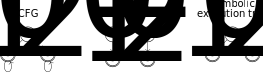
\includegraphics[scale=1.25]{image/execution_branch.pdf}
    \end{center}
    \caption{Control flow graph, execution paths,
        and symbolic execution tree of a program with one branch.}
\end{figure}

\subsublevel{Properties}

$|\mathds{P}_\mathcal{P}| = 2$.
$1 \le |\mathds{P}''_\mathcal{P}| \le 2$.

\sublevel{Simplest cycle program}

\subsublevel{Definition}

Simplest program that contains a cycle:
\begin{itemize}
    \item $\mathcal{P}_{\text{cycle}} = \langle F, D \rangle =
        \langle \{f_0, f_1, f_2\}, D \rangle$,
    \item $f_0^F[D] = \{f_0, f_1\}$. $f_1^F[D] = \{f_1\}$.
\end{itemize}

\begin{figure}[h!]
    \begin{center}
        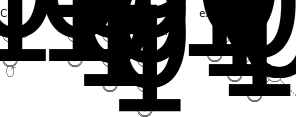
\includegraphics[scale=1.25]{image/execution_cycle.pdf}
    \end{center}
    \caption{Control flow graph, execution paths,
        and symbolic execution tree of a program with one cycle.}
\end{figure}

\subsublevel{Properties}

$|\mathds{P}_\mathcal{P}| = \infty$.
$1 \le |\mathds{P}''_\mathcal{P}|$.

\sublevel{Change data under tainted condition}

\subsublevel{Code snippet}

\lstset{language=c,caption=Listing,label={lst:impl}}
\begin{lstlisting}[numbers=left,numberstyle=\scriptsize]
int a = read();
int b = 0;

if (a) {
    b = 1;
}
if (b == 0) {
    // Point 1.
} else {
    // Point 2.
}
\end{lstlisting}

\subsublevel{Definition}

\sublevel{Table values}

\subsublevel{Code snippet}

\comment{For this one we should have memory indexing.
How can we reach that?}

\lstset{language=c,caption=Listing,label={lst:impl}}
\begin{lstlisting}[numbers=left,numberstyle=\scriptsize]
char* a = read_array();
char* b = init_array();
char* map = {"a...zA...Z"};

for (int i = 0; i < a.length(); i++) {
    if (a[i] > 26) {
        b[i] = map[a[i] - 'a' - 26]
    } else {
        b[i] = a[i];
    }
}
\end{lstlisting}

\comment{It is just write by tainted index.}

\sublevel{SAGE example}

Example from SAGE paper~\cite{sage}.
\lstset{language=c,caption=Listing,label={lst:impl}}
\begin{lstlisting}[numbers=left,numberstyle=\scriptsize]
void top(char input[4]) {
    int cnt=0;
    if (input[0] == 'b') cnt++;
    if (input[1] == 'a') cnt++;
    if (input[2] == 'd') cnt++;
    if (input[3] == '!') cnt++;
    if (cnt >= 3) abort(); // error
}
\end{lstlisting}

This example could be formalized as:
\begin{itemize}
    \item $\mathcal{P}_{\diamond} = \langle F, D \rangle =
        \langle \{f_0, f_1\}, \{x, y, z\} \rangle$,
    \item $x, y \in \mathcal{B} = \{\false, \true\}$,
    \item $f_0 = (f^F_0, f^D_0), f^F_0(\{x, y, z\}) = f_1,
        f^D_0(\{x, y, z\}) = \{x, y, x \diamond y\}$.
    \item $f_1 = (f^F_1, f^D_1), f^F_1(\{x, y, z\}) = f_1,
        f^D_1(\{x, y, z\}) = \{x, y, z\}$.
\end{itemize}

\sublevel{Veritesting example}

Example from Veritesting paper~\cite{veritesting}.
\lstset{language=c,caption=Listing,label={lst:impl}}
\begin{lstlisting}[numbers=left,numberstyle=\scriptsize]
for (int i = 0; i < 100; i++) {
    if (input[i] == 'a') counter++;
}
if (counter == 75) abort();
\end{lstlisting}

\level{Other models}

We compare our model with other concrete, symbolic, and dynamic symbolic
program execution models.

\comment{Add models from:}
\begin{itemize}
    \item A Theory and Practice of Program Development.
        By Derek J. Andrews
    \item Distributed Programming: Theory and Practice.
        By A. Udaya Shankar.
\end{itemize}

\sublevel{Knuth}

In Knuth model~\cite{knuth} program is $\langle Q, I, \Omega, f \rangle$,
where $f: Q \ra Q$, $Q$~--- states, $\Omega$~--- terminal states,
$I$~--- input states.
$\forall x \in I$ path is $x_0, x_1, \dots, x_k, \dots$.
$x_0 = x, x_{k + 1} = f(x_k)$.

\sublevel{Schwartz}

Program model described in~\cite{dta_fse} is based on statements.

\sublevel{Splat}

Splat~\cite{splat} program model is based on labeled statements: $\ell: s$.
Statement is:
\begin{enumerate}[itemsep=-0.5ex]
    \item $\textbf{halt}$, $\textbf{abort}$,
    \item $\textbf{input}(l, k)$, $l$ --- buffer address, $k$ --- size,
    \item $l := e$, $l$ --- address, $e$ --- expression,
    \item $\textbf{if}(e)\,\textbf{goto}\, \ell$, $e$ --- expression,
        $\ell$ --- label,
    \item $l := \textbf{malloc}(k)$, $k$ --- size,
    \item $\textbf{free}(e)$, $e$ --- address.
\end{enumerate}

% \listoffigures
% \listoftables
% \printindex

\bibliography{paper}{}
\bibliographystyle{plain}

\end{document}
